\documentclass[../ut-dissertation.tex]{subfiles}
\begin{document}

\chapter{Results}
This chapter contains the results of two sample runs of the model.
The first is a simple example which is intended to show what the
model's results look like.  The second example is the result of the
classification of a regional conference paper.

\section{A Simple Example}
One of the problems with a model such as this one is that ground truth
is difficult to arrive at.  In fact, this model quantifies a property
which even the author of the documents in question may be unaware of.
As such, verification of the model depends on the sensibility of its
answers.  However, this again presents a challenge because the total
structure of all of the factors and relationships among them is
very complex and difficult to visualize.  To help alleviate this
problem, this section contains a very simple example, one in which all
of the components of the model may be seen.  This example uses three
simple stories, written for this purpose, drawing on a 30 word
vocabulary.  The first story is in Figure~\ref{fig:cat_story}, the
second is in Figure~\ref{fig:dog_story}, and the third is in
Figure~\ref{fig:cat_dog_story}.  The third story is intended to be a
sequel of sorts, drawing on material from the previous stories.  The
complete vocabulary for this example is shown in
Table~\ref{tab:catdog_vocabulary}.
\begin{figure}[p]
  \noindent\fbox{%
    \parbox{\textwidth}{%
     The cat sat on the mat.  The cat was happy to be on the mat.  The cat
     saw the mouse running but was too lazy to chase it.
   }}
  \caption{The Cat's Tale}\label{fig:cat_story}
\end{figure}

\begin{figure}[p]
  \noindent\fbox{%
    \parbox{\textwidth}{%

    The dog walked to the house.  The dog saw the food bowl, and the
    dog saw a squirrel.  The dog chased the squirrel from the food
    bowl.
  }}
  \caption{The Dog's Tale}\label{fig:dog_story}
\end{figure}

\begin{figure}[p]
  \noindent\fbox{%
    \parbox{\textwidth}{%
    The dog saw the cat on the mat.  The dog walked to the house, and
    the dog chased the cat.  The squirrel was happy to see the dog
    chase the cat on the mat.  The dog saw the squirrel, and decided
    to chase the squirrel instead.  The cat sat on the mat.
}}
  \caption{The Saga Continues}\label{fig:cat_dog_story}
\end{figure}

\begin{table}[p]
  \centering
  \caption{Cat and Dog Vocabulary}\label{tab:catdog_vocabulary}
  \begin{tabular}{|c|l||c|l|}
    \hline
    $I$ & Word & $I$ & Word\\ 
    \hline
    1 & the & 16 & chased \\
    2 & house & 17 & sat \\
    3 & mouse & 18 & be \\
    4 & squirrel & 19 & happy \\
    5 & it & 20 & on\\
    6 & saw & 21 & from \\
    7 & lazy & 22 & food \\
    8 & cat & 23 & decided \\
    9 & mat & 24 & to\\
   10 & a & 25 & was \\
   11 & bowl & 26 & dog \\
   12 & walked & 27 & running \\
   13 & too & 28 & instead \\
   14 & and & 29 & but \\
   15 & see & 30 & chase\\
    \hline
  \end{tabular}
\end{table}
\FloatBarrier

The number of factors was determined by trial decomposition of the
target document.  The target document consists of 52 words, which
yields 49 3-grams of which 42 are unique.  The resultant document
tensor has 42 non-zero entries.  Of course, one unique solution to the
decomposition of this tensor would be 42 tensors consisting of the
individual non-zero entries in the same position as in the target
tensor.  This would be the maximal candidate for the rank of the
tensor.  Tensor decompositions were performed for between 1 and 42
factors.  Above 15 factors, the CCD algorithm produced factorizations
that were mostly zeroes.  That is, most of factor tensors consisted
entirely of zero entries.  This is due to the small number of entries
present, and the small amount of variation between them.  Because the
higher-ranked factorizations all suffered from this problem, they were
excluded for consideration.  For the factorizations between 1 and 15
factors, 7 yielded the best fit with an error ratio of 0.45, and so 7
was determined to be the optimal number of factors for this
corpus. Even with this relatively poor fit, the model was able to
distinguish features of the stories.  The distances between the
factors, other than the diagonals, range from 0 to 1.4.  The final
classification step yielded the classification of factors shown in
Table~\ref{tab:cat_dog_class}.

The model threshold value was set to 0.2, which is a sensible value as
this requires a 90\% match in a factor.  In this case it would not
have mattered, however, as the matching factors were all perfect
matches with an $L_1$ distance of 0.

\begin{table}[p]
  \centering
  \caption{Cat Dog Model} \label{tab:cat_dog_class}
  \begin{tabular}{|l|c|l|}
    \hline
    Factor & Factor Weight & Classification\\
    \hline
    1 & 0.28 & Author Contribution\\
    2 & 0.15 & Cat Factor 1\\
    3 & 0.14 & Author Contribution\\
    4 & 0.14 & Author Contribution\\
    5 & 0.11 & Author Contribution\\
    6 & 0.11 & Author Contribution\\
    7 & 0.06 & Dog Factor 1\\
    \hline
  \end{tabular}
\end{table}


Factor two was matched to the cat story, and factor seven was matched
to the dog story.  These factors are shown in
Table~\ref{tab:catfactor} and Table~\ref{tab:dogfactor}.  The
remaining factors (1,3,4,5, and 6) were determined to be original to
the target document.  These factors are seen in
Table~\ref{tab:sequel_original}.

\begin{table}[p]
  \centering
  \caption{Factor 2 - Matched to Cat Factor 1}\label{tab:catfactor}
  \begin{tabular}{|lll|r|}
    \hline
    Word 1 & Word 2 & Word 3 & Proportion\\
    \hline
    on & the & mat & 1.00\\
    \hline
  \end{tabular}
\end{table}

\begin{table}[p]
  \centering
  \caption{Factor 7 - Matched to Dog Factor 1}\label{tab:dogfactor}
  \begin{tabular}{|lll|r|}
    \hline
    Word 1 & Word 2 & Word 3 & Proportion\\
    \hline
    the & dog & saw & 0.40\\
    the & dog & walked & 0.20\\
    the & dog & chased & 0.20\\
    the & dog & chase & 0.20\\
    \hline
  \end{tabular}
\end{table}

\begin{table}[p]
  \centering
  \caption{Sequel Original Factors}\label{tab:sequel_original}
  \begin{tabular}{|lll|r|}
    \hline
    Word 1 & Word 2 & Word 3 & Proportion \\
    \hline
    saw & the & squirrel & 0.267417\\
    saw & the & cat & 0.223651\\
    saw & the & dog & 0.192194\\
    cat & the & squirrel & 0.044066\\
    cat & the & cat & 0.036854\\
    cat & the & dog & 0.031670\\
    mat & the & squirrel & 0.034331\\
    mat & the & cat & 0.028712\\
    mat & the & dog & 0.024674\\
    see & the & squirrel & 0.032132\\
    see & the & cat & 0.026873\\
    see & the & dog & 0.023094\\
    chased & the & squirrel & 0.013437\\
    chased & the & cat & 0.011238\\
    chased & the & dog & 0.009657\\
    \hline
    squirrel & and & happy & 0.249836\\
    squirrel & and & decided & 0.262960\\
    squirrel & was & happy & 0.237368\\
    squirrel & was & decided & 0.249836\\
    \hline
    decided & to & chase & 1.000000\\
    \hline
    happy & to & see & 1.000000\\
    \hline
    cat & saw & the & 0.345830\\
    cat & see & the & 0.040819\\
    cat & chased & the & 0.172914\\
    cat & chase & the & 0.213734\\
    walked & saw & the & 0.056987\\
    walked & see & the & 0.006726\\
    walked & chased & the & 0.028493\\
    walked & chase & the & 0.035220\\
    to & saw & the & 0.044398\\
    to & see & the & 0.005240\\
    to & chased & the & 0.022199\\
    to & chase & the & 0.027439\\
    \hline
  \end{tabular}
\end{table}

The separation that the model accomplished, even with very scant data,
shows that the expected similarities in the resultant factors are
present.  The next step is to look at a more substantial example.
\FloatBarrier

\section{A Conference Paper Case Study}
For a real-world case study, a conference paper was pulled from the
ACM Digital library.  This was the first paper listed in the first
conference listed in their regional conference proceedings.  This
paper cites four other papers and two websites.  The two websites were
used to pull data, and so they are not included in the corpus.  In
addition to the four cited papers, two unrelated papers are included
to test if the model will select factors from these unrelated papers.
The complete corpus, listed with the target paper last, is shown in
Table~\ref{tab:conference_corpus}. Documents 1-4 are the papers cited
by the target paper, documents 5-6 are unrelated papers, and document
7 is the target paper.

\begin{table}[p]
  \centering
  \caption{Conference Paper Corpus}\label{tab:conference_corpus}
  \begin{tabular}{|l|l|}
    \hline
    Num & Document Information\\
    \hline
    1 & Jessica Lin, Eamonn Keogh, Stefano Lonardi, and Bill Chiu. A\\
      & symbolic representation of time series, with implications for\\
      & streaming algorithms. In Proc. DMKD 2003, pages 2–11. ACM
        Press, 2003.\\
    \hline
    2 & Andreas Schlapbach and Horst Bunke. Using hmm\\
      & based recognizers for writer identification and\\
      & verification. In Proc. FHR 2004, pages 167–172. IEEE, 2004.\\
    \hline
    3 & Yusuke Manabe and Basabi Chakraborty. Identity\\
      & detection from on-line handwriting time series. In Proc.\\
      & SMCia 2008, pages 365–370. IEEE, 2008.\\
    \hline
    4 & Sami Gazzah and Najoua Ben Amara. Arabic \\
      & handwriting texture analysis for writer identification\\
      & using the dwt-lifting scheme. In Proc. ICDAR 2007,\\
      & pages 1133–1137. IEEE, 2007.\\
    \hline
    5 & Kolda, Tamara Gibson. Multilinear operators for higher-order \\
      & decompositions. 2006\\
    \hline
    6 & Blei, David M and Ng, Andrew Y and Jordan, Michael I. Latent\\
      & dirichlet allocation. 2007\\
    \hline
    7 & Serfas, Doug. Dynamic Biometric Recognition of Handwritten Digits\\
      & Using Symbolic Aggregate Approximation. Proceedings of the ACM\\
      & Southeast Conference 2017\\
    \hline
  \end{tabular}
\end{table}

The entire corpus consists of 45,152 words.  As described in the
previous chapter, the vocabulary was truncated to 600 words.  The 600
words were the most frequent words across the corpus.  The other
parameters are shown in Table~\ref{tab:model_parameters}
\begin{table}[p]
  \centering
  \caption{Conference Model Parameters}\label{tab:model_parameters}
  \begin{tabular}{ccc}
    \hline
    $n$ & $nfactors$ & $threshold$\\
    \hline
    3 & 150 & 0.2\\
    \hline
  \end{tabular}
\end{table}
\end{document}
Again, 0.2 is used as the threshold as it is a good default setting.
The decomposition of the 7 documents into 150 factors was carried out
on a machine with a 3.9GHz 8-core Intel processor and 15GB of RAM.
The decomposition and construction of normalized tensors took
approximately 2.5 hours to complete. Calculation of the distance
matrix and classifying the factors required another hour and a half.
The results are shown in Table~\ref{tab:conference_results}.

The distribution of the factor distances are shown in
Figure~\ref{fig:conference_distribution}.  The vertical red line on
the graphs shows the threshold for factor matching.
Figure~\ref{fig:conference_distribution}(a) shows the distribution of
factor distances for the entire factor matrix while
~\ref{fig:conference_distribution}(b) shows the distribution of
the distances from the target factors.  Note that both distributions
are tri-modal.  The two spikes on the far left correspond to factors
from the unrelated documents, which shows that they are well separated
from the target document's factors.


\begin{table}[p]
  \centering
  \caption{Conference Classification Results}\label{tab:conference_results}
  \begin{tabular}{|l|c|l|}
    \hline
    Document & Influence & Number of Matched Factors\\
    \hline
    1 & 0.21 & 10\\
    2 & 0.09 & 9\\
    3 & 0.06 & 3\\
    4 & 0.06 & 1\\
    5 & 0.00 & 0\\
    6 & 0.00 & 0\\
    Author & 0.57 & 127\\
    \hline
  \end{tabular}
\end{table}

\begin{figure}[p]
  \centering
  \subfloat[All Factor Distances]{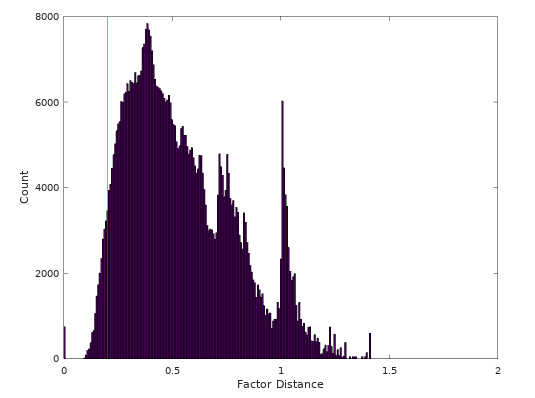
\includegraphics[width=3in]{diagrams/conference-factor-distance}}
  \subfloat[Target Factor
  Distances]{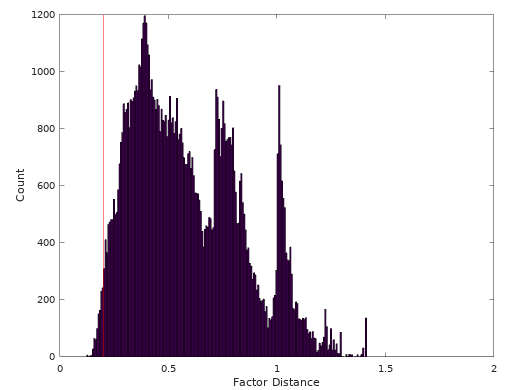
\includegraphics[width=3in]{diagrams/conference-target-distance}}
    \caption{Factor Distance Distribution}\label{fig:conference_distribution}
\end{figure}
\FloatBarrier

\begin{table}[p]
  \centering
  \caption{First 30 Non-Zero Entries of Factor 56}\label{fig:factor-56}
  \begin{tabular}{|lll|r|}
    \hline
    Word 1 & Word 2 & Word 3 & Proportion\\
    \hline
    is & the & sax & 0.000887\\
    into & the & data & 0.000886\\
    symbols & the & sax & 0.000874\\
    digits & the & timeseries & 0.000865\\
    digits & the & data & 0.000857\\
    with & the & sax & 0.000856\\
    from & the & square & 0.000852\\
    however & the & sax & 0.000844\\
    up & the & sax & 0.000844\\
    characters & the & sax & 0.000844\\
    becomes & the & sax & 0.000844\\
    note & the & sax & 0.000843\\
    using & the & sax & 0.000841\\
    for & the & square & 0.000838\\
    into & the & sax & 0.000838\\
    from & the & svc & 0.000833\\
    from & the & paa & 0.000832\\
    author & the & square & 0.000828\\
    on & the & author & 0.000824\\
    for & the & svc & 0.000819\\
    for & the & paa & 0.000818\\
    on & the & accuracy & 0.000814\\
    on & the & array & 0.000814\\
    digits & the & sax & 0.00081\\
    author & the & svc & 0.000809\\
    author & the & paa & 0.000808\\
    on & the & distance & 0.000806\\
    on & the & x & 0.000806\\
    from & the & timeseries & 0.000804\\
    of & the & author & 0.000802\\
    \hline
  \end{tabular}
\end{table}

  

As these results show, the model makes a set of reasonable matches,
and it does not select unrelated documents.  The actual makeup of the
factors are much more complex, however ideas can be traced through
them.  Unfortunately, these factors are much too large to be included
verbatim in this chapter. However, the factors that were matched from
paper one all deal with a technique which generates a symbolic
representation of a time series.  This technique serves as the basis
for the invention in the paper, and is talked about many times with
many of the same explanations used in the first paper.  Thus the model
has not only avoided unrelated information, it has given a greater
weight to the paper which had the greatest semantic influence on the
work being studied.
